\documentclass[oneside,final,12pt]{extarticle}
%\documentclass[oneside,draft,12pt]{extarticle}
\usepackage[unicode]{hyperref}
\hypersetup{draft=false,bookmarksnumbered,bookmarksopen}
\usepackage{cmap}
\usepackage[T2A]{fontenc}
\usepackage[utf8]{inputenc}
\usepackage[russian]{babel}
\usepackage{vmargin}
\setpapersize{A4}
\setmarginsrb{3cm}{2cm}{1.5cm}{2cm}{0pt}{0mm}{0pt}{13mm}
\usepackage{indentfirst}
\sloppy % Предотвращает вылезание строки за правый край.
%\fussy % Строки будут вылазить за правый край.
\usepackage{graphicx}
\usepackage{setspace}
\onehalfspacing
\clubpenalty=9999
\widowpenalty=9999
\usepackage{amsfonts}
\usepackage{amsmath}
\usepackage{color}
\usepackage{enumitem}
\usepackage{listings}
\lstdefinelanguage{MyLang}{morekeywords={storebe, loadbe,loadi, rol, orbe, subi, cmpj,cmpjn,cmpjg,cmpjl, j, tree_lpm, tree_in},sensitive=false,morecomment=[l]{//},morecomment=[s]{/*}{*/},morestring=[b]",}
\lstdefinelanguage{Pseudo}{morekeywords={procedure,if,endif,for,else,then,not,all,in,do,endfor},sensitive=false,morecomment=[l]{//},morecomment=[s]{/*}{*/},morestring=[b]",}
\lstset
{language=MyLang,frame=tb,
 extendedchars=true,escapechar=',
 commentstyle=\itshape,
 numbers=left,
 basicstyle=\footnotesize\ttfamily,
 keywordstyle=\footnotesize\ttfamily\bf,
 xleftmargin=20pt,
 xrightmargin=20pt,}
 
\begin{document}

\bibliographystyle{ugost2008}
%\bibliographystyle{gost780}
%\bibliographystyle{ugost2003s}
\title{Анализ поведения пользователей для предотвращения инсайдерских угроз}
\author{Калякина Алина Дмитриевна}

\makeatletter
\renewcommand\@maketitle{
	\begin{titlepage}
		\begin{center}
			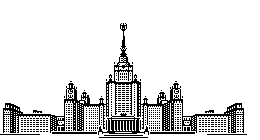
\includegraphics{msu} \\
		Московский государственный университет имени М.\,В. Ломоносова
			\\
			Факультет вычислительной математики и кибернетики \\
			Кафедра автоматизации систем вычислительных комплексов \\
			
			\vspace{8em}
			
			{\Large \@author} \\[1.5em]
			{\LARGE \textbf{\@title} \par}
			
			\vspace{4.5em}
			
			{\Large \textsc{курсовая работа}}
			
			\vfill
			
			\begin{flushright}
				{\large
					\textbf{Научный руководитель}:\\
					к.\,ф.-м.\,н., ???\\
					Д.\,В.~Царёв\\
					\vspace{0.2em}
				}
			\end{flushright}
			\vfill
			
			Москва, 2020
		\end{center}
	\end{titlepage}
}
\makeatother

\maketitle
\setcounter{page}{2}


\section*{Аннотация}
Тут будет аннотация
\clearpage
\tableofcontents
\clearpage
\section{Введение}
Тут будет введение
\clearpage
\section{Постановка задачи}
Формальная постановка задачи звучит следующим образом:
\begin{enumerate}
\item Исследовать и разработать методы обнаружения инсайдерских атак с использованием методов машинного обучения
\item Предложенный метод проверить для следующих сценариев:
\begin{itemize}
\item 1
\item 2.
\end{itemize}
\item Использовать контент
\end{enumerate}
\clearpage
\section{Обзор существующих решений рассматриваемой зада­чи или ее модификаций}
Рассмотрим существующие методы обнаружения инсайдерских угроз, сделаем их сравнение. Обратим особое внимание на использование контентной составляющей поведения пользователей, сравним используемые в различных работах подходы. В конце, рассмотрим существующие для наддной работы наборы данных.
\subsection{Обзор существующих подходов}
Задача обнаружения инсайдерских угроз может быть рассмотрена с двух ракурсов: как задача поиска аномалий, и как задача обучения с учителем.
В первом случае...
Сравнение работ по критериям:
\begin{enumerate}
\item Supervised/unsupervised
\item Количество ''этапов''
\item Использование контекста
\item Использование контента
\item Использованные наборы данных
\item Качество на CERT
\end{enumerate}
Сравнение самих моделей??? (это есть в ревью, но не факт, что полезно)
\begin{enumerate}
\item One-class SVM
\item Random Forest
\item ...
\end{enumerate}
\subsection{Подходы к работе с контентом}
ABSA - анализ, LDA, эмбеддинги. Как это работает примеры работ с этим.
\subsection{Обзор наборов данных}
\clearpage


\clearpage
\bibliography{biblio}
\addcontentsline{toc}{section}{Список литературы}

\clearpage
\end{document}
